% Once your paper is accepted for publication,                                                                                                                                         
% PLEASE REMOVE ALL TRACKED CHANGES in this file                                                                                                                                       
% and leave only the final text of your manuscript.                                                                                                                                    
% PLOS recommends the use of latexdiff to track changes during review, as this will help to maintain a clean tex file.                                                                 
% Visit https://www.ctan.org/pkg/latexdiff?lang=en for info or contact us at latex@plos.org.                                                                                           

% Please do not include colors or graphics in the text.
%
% The manuscript LaTeX source should be contained within a single file (do not use \input, \externaldocument, or similar commands).
%
% % % % % % % % % % % % % % % % % % % % % % %
%
% -- FIGURES AND TABLES
%
% Please include tables/figure captions directly after the paragraph where they are first cited in the text.
%
% DO NOT INCLUDE GRAPHICS IN YOUR MANUSCRIPT
% - Figures should be uploaded separately from your manuscript file. 
% - Figures generated using LaTeX should be extracted and removed from the PDF before submission. 
% - Figures containing multiple panels/subfigures must be combined into one image file before submission.
% For figure citations, please use "Fig" instead of "Figure".
% See http://journals.plos.org/plosone/s/figures for PLOS figure guidelines.
%
% Tables should be cell-based and may not contain:
% - spacing/line breaks within cells to alter layout or alignment
% - do not nest tabular environments (no tabular environments within tabular environments)
% - no graphics or colored text (cell background color/shading OK)
% See http://journals.plos.org/plosone/s/tables for table guidelines.
%
% For tables that exceed the width of the text column, use the adjustwidth environment as illustrated in the example table in text below.
%
% % % % % % % % % % % % % % % % % % % % % % % %
%
% -- EQUATIONS, MATH SYMBOLS, SUBSCRIPTS, AND SUPERSCRIPTS
%
% IMPORTANT
% Below are a few tips to help format your equations and other special characters according to our specifications. For more tips to help reduce the possibility of formatting errors during conversion, please see our LaTeX guidelines at http://journals.plos.org/plosone/s/latex
%
% For inline equations, please be sure to include all portions of an equation in the math environment.  For example, x$^2$ is incorrect; this should be formatted as $x^2$ (or $\mathrm{x}^2$ if the romanized font is desired).
%
% Do not include text that is not math in the math environment. For example, CO2 should be written as CO\textsubscript{2} instead of CO$_2$.
%
% Please add line breaks to long display equations when possible in order to fit size of the column. 
%
% For inline equations, please do not include punctuation (commas, etc) within the math environment unless this is part of the equation.
%
% When adding superscript or subscripts outside of brackets/braces, please group using {}.  For example, change "[U(D,E,\gamma)]^2" to "{[U(D,E,\gamma)]}^2". 
%
% Do not use \cal for caligraphic font.  Instead, use \mathcal{}
%
% % % % % % % % % % % % % % % % % % % % % % % % 
%
% Please contact latex@plos.org with any questions.
%
% % % % % % % % % % % % % % % % % % % % % % % %

\documentclass[10pt,letterpaper]{article}

\usepackage[top=0.85in,left=2.75in,footskip=0.75in]{geometry}

% amsmath and amssymb packages, useful for mathematical formulas and symbols
\usepackage{amsmath,amssymb}

% Use adjustwidth environment to exceed column width (see example table in text)
\usepackage{changepage}

% textcomp package and marvosym package for additional characters
\usepackage{textcomp,marvosym}

% cite package, to clean up citations in the main text. Do not remove.
\usepackage{cite}

% Use nameref to cite supporting information files (see Supporting Information section for more info)
\usepackage{nameref,hyperref}

% line numbers
\usepackage[right]{lineno}

% ligatures disabled
\usepackage[nopatch=eqnum]{microtype}
\DisableLigatures[f]{encoding = *, family = * }

% color can be used to apply background shading to table cells only
\usepackage[table]{xcolor}

% array package and thick rules for tables
\usepackage{array}

% create "+" rule type for thick vertical lines
\newcolumntype{+}{!{\vrule width 2pt}}

% create \thickcline for thick horizontal lines of variable length
\newlength\savedwidth
\newcommand\thickcline[1]{%
  \noalign{\global\savedwidth\arrayrulewidth\global\arrayrulewidth 2pt}%
  \cline{#1}%
  \noalign{\vskip\arrayrulewidth}%
  \noalign{\global\arrayrulewidth\savedwidth}%
}

% \thickhline command for thick horizontal lines that span the table
\newcommand\thickhline{\noalign{\global\savedwidth\arrayrulewidth\global\arrayrulewidth 2pt}%
\hline
\noalign{\global\arrayrulewidth\savedwidth}}


% Remove comment for double spacing
%\usepackage{setspace} 
%\doublespacing

% Text layout
\raggedright
\setlength{\parindent}{0.5cm}
\textwidth 5.25in 
\textheight 8.75in

% Bold the 'Figure #' in the caption and separate it from the title/caption with a period
% Captions will be left justified
\usepackage[aboveskip=1pt,labelfont=bf,labelsep=period,justification=raggedright,singlelinecheck=off]{caption}
\renewcommand{\figurename}{Fig}

% Use the PLoS provided BiBTeX style
\bibliographystyle{plos2015}

% Remove brackets from numbering in List of References
\makeatletter
\renewcommand{\@biblabel}[1]{\quad#1.}
\makeatother



% Header and Footer with logo
\usepackage{lastpage,fancyhdr,graphicx}
\usepackage{epstopdf}
%\pagestyle{myheadings}
\pagestyle{fancy}
\fancyhf{}
%\setlength{\headheight}{27.023pt}
%\lhead{\includegraphics[width=2.0in]{PLOS-submission.eps}}
\rfoot{\thepage/\pageref{LastPage}}
\renewcommand{\headrulewidth}{0pt}
\renewcommand{\footrule}{\hrule height 2pt \vspace{2mm}}
\fancyheadoffset[L]{2.25in}
\fancyfootoffset[L]{2.25in}
\lfoot{\today}

%% Include all macros below

\newcommand{\lorem}{{\bf LOREM}}
\newcommand{\ipsum}{{\bf IPSUM}}

%% END MACROS SECTION

%% BEGIN PPSE SECTION
% \usepackage[utf8]{inputenc}
% \usepackage{amsmath}
% \usepackage{amsfonts}
% \usepackage{amssymb}
% \usepackage{mathrsfs}
\usepackage{amsthm}
% \usepackage{graphicx}
% \usepackage{caption}
\usepackage{listings}
% \usepackage{natbib}
% \usepackage{xcolor}
% \usepackage{hyperref}


% %\bibliographystyle{jtbnew}
% \setcitestyle{authoryear,round,aysep={}}

\theoremstyle{definition}
\newtheorem*{df*}{Definition} 

\theoremstyle{remark}
\newtheorem*{nt*}{Note}

\usepackage{color}
\newcommand{\red}[1]{\textcolor{red}{#1}}
\newcommand{\blue}[1]{\textcolor{blue}{#1}}

\lstdefinelanguage{scala}{morekeywords={class,object,trait,extends,with,new,if,while,for,def,val,var,this},
otherkeywords={->,=>},
sensitive=true,
morecomment=[l]{//},
morecomment=[s]{/*}{*/},
morestring=[b]"}

% Default settings for code listings
\lstset{frame=tb,language=scala,aboveskip=3mm,belowskip=3mm,showstringspaces=false,breaklines=true,basicstyle=\ttfamily\footnotesize,numberstyle=\footnotesize,numbers=left, stepnumber=1,xleftmargin=10pt }
%% END PPSE SECTION


\begin{document}
\vspace*{0.2in}

% Title must be 250 characters or less.
\begin{flushleft}
{\Large
  \textbf\newline{A new method to evaluate simulation models: The Pattern Probability Space Estimation (PPSE) algorithm} % Please use "sentence case" for title and headings (capitalize only the first word in a title (or heading), the first word in a subtitle (or subheading), and any proper nouns).
}
\newline
% Insert author names, affiliations and corresponding author email (do not include titles, positions, or degrees).
\\
Romain Reuillon\textsuperscript{1\Yinyang*},
Julien Perret\textsuperscript{2\Yinyang}
% Name3 Surname\textsuperscript{2,3\textcurrency},
% Name4 Surname\textsuperscript{2},
% Name5 Surname\textsuperscript{2\ddag},
% Name6 Surname\textsuperscript{2\ddag},
% Name7 Surname\textsuperscript{1,2,3*},
% with the Lorem Ipsum Consortium\textsuperscript{\textpilcrow}
\\
\bigskip
\textbf{1} Géographie-Cités, CNRS, Paris, France, ISC-PIF, Paris, France
\\
\textbf{2} LASTIG, Univ Gustave Eiffel, IGN, ENSG, Saint-Mande, France
\\
% \textbf{3} Affiliation Dept/Program/Center, Institution Name, City, State, Country
% \\
\bigskip

% Insert additional author notes using the symbols described below. Insert symbol callouts after author names as necessary.
% 
% Remove or comment out the author notes below if they aren't used.
%
% Primary Equal Contribution Note
\Yinyang These authors contributed equally to this work.

% Additional Equal Contribution Note
% Also use this double-dagger symbol for special authorship notes, such as senior authorship.
% \ddag These authors also contributed equally to this work.

% Current address notes
% \textcurrency Current Address: Dept/Program/Center, Institution Name, City, State, Country % change symbol to "\textcurrency a" if more than one current address note
% \textcurrency b Insert second current address 
% \textcurrency c Insert third current address

% Deceased author note
% \dag Deceased

% Group/Consortium Author Note
% \textpilcrow Membership list can be found in the Acknowledgments section.

% Use the asterisk to denote corresponding authorship and provide email address in note below.
* romain.reuillon@iscpif.fr

\end{flushleft}
% Please keep the abstract below 300 words
\section*{Abstract}
Lorem ipsum dolor sit amet, consectetur adipiscing elit. Curabitur eget porta erat. Morbi consectetur est vel gravida pretium. Suspendisse ut dui eu ante cursus gravida non sed sem. Nullam sapien tellus, commodo id velit id, eleifend volutpat quam. Phasellus mauris velit, dapibus finibus elementum vel, pulvinar non tellus. Nunc pellentesque pretium diam, quis maximus dolor faucibus id. Nunc convallis sodales ante, ut ullamcorper est egestas vitae. Nam sit amet enim ultrices, ultrices elit pulvinar, volutpat risus.


% Please keep the Author Summary between 150 and 200 words
% Use first person. PLOS ONE authors please skip this step. 
% Author Summary not valid for PLOS ONE submissions.   
% \section*{Author summary}
% Lorem ipsum dolor sit amet, consectetur adipiscing elit. Curabitur eget porta erat. Morbi consectetur est vel gravida pretium. Suspendisse ut dui eu ante cursus gravida non sed sem. Nullam sapien tellus, commodo id velit id, eleifend volutpat quam. Phasellus mauris velit, dapibus finibus elementum vel, pulvinar non tellus. Nunc pellentesque pretium diam, quis maximus dolor faucibus id. Nunc convallis sodales ante, ut ullamcorper est egestas vitae. Nam sit amet enim ultrices, ultrices elit pulvinar, volutpat risus.

\linenumbers

% Use "Eq" instead of "Equation" for equation citations.
\section*{Introduction}

% \begin{abstract}

%Models of social systems generally contain free parameters that cannot be evaluated directly from data. A calibration phase is therefore necessary to assess the capacity of the model to produce the expected dynamics. However, despite the high computational cost of this calibration it doesn't produce a global picture of the relationship between the parameter space and the behaviour space of the model. The Calibration Profile (CP) algorithm is an innovative method extending the concept of automated calibration processes. It computes a profile that depicts the effect of each single parameter on the model behaviour, independently from the others. A 2-dimensional graph is thus produced exposing the impact of the parameter under study on the capacity of the model to produce expected dynamics. The first part of this paper is devoted to the formal description of the CP algorithm. In the second part,we apply it to an agent based geographical model (SimpopLocal). The analysis of the results brings to light novel insights on the model.

% \noindent
% \textbf{Keywords:} calibration profile, model evaluation, agent based modelling

% \end{abstract}

%\author[geoc,isc]{Romain Reuillon}
%\author[geoc,isc]{Clara Schmitt}
%\author[isc]{Ricardo De Aldama}
%\author[isir]{Jean-Baptiste Mouret}
%\address[geoc]{Géographie-cités - UMR 8504\\13 rue du Four\\75006 Paris}
%\address[isc]{Institut des Systémes Complexes\\11 place Nationale\\75013 Paris}
%\address[isir]{'Institut des Systèmes Intelligents et de Robotique (ISIR) - UMR7222\\4 place Jussieu 75252\\Paris cedex 05}

% \title{A new method to evaluate simulation models: The Pattern Probability Space Estimation (PPSE) algorithm}

% \maketitle
%
%Agent-based modelling is widely used in models of social systems because it is well suited to describe individual-centred dynamics with non-linear interactions. This modelling technique, however, introduces many free parameters which critically influence the behaviour of the model. Hand-picking parameters is a time-consuming process and makes it hard to evaluate the ability of a model to reproduce empirical data or formalised knowledge. Automatic calibration of models have the potential to free the modeller from the time-consuming process of finding parameters and to make the modelling process more rigorous by reducing the number of arbitrary choices.
%
%The current prevalent method for automatic calibration is to see it as an optimization problem in which the differences between known data and model predictions have to be minimized. This optimization can be performed with different optimization algorithms like "Adaptive Bayesian  Calibration" \citep{Lenormand2012} or evolutionary algorithms \citep{Stonedahl2011, schmitt2014}. Nevertheless, these methods find a single set of parameters, or, in the case of the multi-objective evolutionary algorithms, a set of parameters that represent optimal trade-off with regard to several model quality criteria. In both cases, the result of the calibration is solely that the model \emph{can} reproduce the data with a given precision. These calibration processes does not say anything about how often parameter sets lead to realistic behaviours, and about how a each parameter will change the behaviour of the model. For instance, in it is often interesting to know when some parameter values would prevent the system to reach a realistic behaviour, rather than only knowing a singles set of "optimal" parameter values.
%
%To compute a more global view of the parameter space, we have therefore designed a novel method that exposes the sensitivity of a single parameter on the calibration of a model independently of the other parameters. A high level representation of this method is shown on Figure \ref{globalpicture}. It computes the lowest calibration error that can possibly be obtained when the value of a given parameter is fixed and the other are free. It computes this minimal error for many values of the parameter under study. The value of the parameter are sampled all along its domain of definition to produce a so called \emph{calibration profile}. For each sample value, the value of the remaining parameters are optimised in order to find the lowest possible calibration error. The profile can then be drawn on a $2$-dimensional chart that depicts the influence of the parameter under study on the model calibration.
%
%\begin{figure}
% \centering
%  \includegraphics[width=1\linewidth]{globalpicture.pdf}
% \captionof{figure}{ \label{globalpicture} High level representation of the Calibration Profile (CP) method }
%\end{figure}
%
%To produce such a profile, a naive approach would consist in executing an entire calibration algorithm for each value of the parameter under study. Current automated calibration algorithms are too computationally intensive to make this approach tractable in practice. To tackle this problem we have designed an algorithm which computes the numerous points composing a calibration profile altogether (this methods has been inspired by the recently published MOLE method \citep{Mouret2012, Clune2013}, which computes two dimensional maps of phenotype landscapes using evolutionary algorithms). The method, called CP (Calibration Profile) is designed to draw one dimension profiles for model calibration.
%
%The first section of this paper exposes a formal description of the CP algorithm as well as a reusable implementation of method. In the second section we show how the application of the CP algorithm to a real world geographical simulation model produces novel insights toward the validation of the model.

% \section{Opening remarks}

In this paper, we choose to expose the PPSE algorithm using purely functional Scala 3 code, that is ready to compile and execute.
The codding has been made as high level and understandable as possible while keeping correct Scala syntax.
Some functions of the Scala standard library are used, especially for collections types.
The documentation for these function is available on the Scala site\footnote{\url{https://scala-lang.org/api/3.x/}}.

All function inputs are passed as parameter, it can call other function, it doesn't have side effects and what the function produces is provided to the calling function through the return value. The code excerpts figured in the paper, are part of a complete implementation of the algorithm available has free software here: {\color{red} url du dépot} 


% \section{Objective}\label{sec. objective}

The PPSE method is inspired from the evolutionary algorithm. It extends the PSE method (citation). The PSE method discovers all the pattern that could be produced by a model given some uncertainty on its parameters. In PSE the pattern space is defined as discrete space containing descriptors of the dynamics of the simulation. Each combination values of these descriptors is considered a distinct pattern.

PSE discovers all the possible patterns, however it does not provide any additional information on these pattern apart from there existence. PPSE extends on that to compute a likelihood for each pattern. PPSE computes the likelihood that the model produce a given pattern when the input parameters are drawn from a uniform distribution.

Lets consider a simulation model and a function that computes patterns from the dynamics produced by the model. The model has some free parameters. For the sake of simplicity we consider here that the input parameters of the model are defined on $[0, 1]$.

\begin{lstlisting}[caption={Model and pattern signatures},label={lst:pattern}]
type Dynamic = ...
type Pattern = Vector[Int]

class Model(compute: Vector[Double] => Dynamic, dimension: Int)

def simulation(model: Model): Dynamic = ...
def pattern(dynamic: Dynamic): Pattern = ...
\end{lstlisting}

The naive algorithm to compute the likelihood of the pattern is to uniformly sample the parameter space and to measure the number of time a given pattern has been reached. 

\begin{lstlisting}[caption={Naive PPSE},label={lst:naivePPSE}]

def naivePPSE(model: Model, pattern: Dynamic => Pattern, random: Random, samples: Int): Map[Pattern, Double] = 
  var patterns = Map[Pattern, Double]()
  
  for 
    i <- 0 to samples
  dor
    val x = Vector.fill(model.dimension)(random.nextDouble())
    val p = pattern(model.compute(x))
    patterns = patterns.getOrElse(p, 0) + 1
  
  val total = patterns.values.sum
  patterns.mapValues(x => x / total)
\end{lstlisting}

This algorithm computes an approximation of the probability to reach a pattern given a uniform sampling of the parameter space. This method is however highly inefficient for model in which a large variability of the dynamics is generated by a very small faction of the input space. This is generally the case in complex systems models. As we have shown in the PSE paper sampling uniformly is, for instance, very inefficient to discovers new patterns in the case of the Reynolds Flocking model.

The idea behind the PPSE algorithm is to evolutionally bias the sampling of the parameter space towards the part generating rare patterns, while keeping the enough knowledge on this bias to be de-bias the results and obtain unbiased estimator of the pattern likelihoods.



{\color{red} Justification methodo, c'est bien de savoir pour un modèle si un pattern est rare ou est commun. Dans le cadre de l'aide à la décision avec PSE on veut savoir si les pattern possible issues de l'incertitude sur le modéle et qui ammène à des cas catastophique sont rares ou pas} 


%The CP method takes inspiration from evolutionary algorithms to provide a thorough analysis of 
%the role played by each parameter. Such analysis is independent from one parameter to the other.
%A function that evaluates the performance of each particular model is supposed to be given
%(typically such evaluation takes into account the fitting of the model to the data). 
%
%Let $\mathcal{M}$ be the set of possible models under consideration and let 
%$A = A_1 \times \ldots \times A_{n} \subseteq \mathbb{R}^n$ be the domain of the parameter vectors that 
%we consider as determining the models, where $n$ is the number of parameters. We denote by  
%$\mu: A \rightarrow \mathcal{M}$ the map that provides a model for a given 
%parameter vector. Such map can be viewed as a meta-model, that is a model with free parameters. 
%
%Let $\tilde{f} : \mathcal{M} \rightarrow \mathbb{R}_{\geq 0}$ be the function providing an evaluation for 
%each model. We can obviously evaluate a 
%parameter vector with the function $f = \tilde{f}\circ \mu : A \rightarrow \mathbb{R}_{\geq 0}$. In this context, when 
%we use the word \emph{solution} we just mean a parameter vector $\bar{a}\in A$. 
%By convention we suppose that best solutions are closer to $0$.
%
%
%To estimate the impact of the $k$-th parameter on the model, we consider the function $h_k: A_k \rightarrow \mathbb{R}$ 
%defined by
%
%$$
%h_k(x) = \inf\{f (a_1\ldots, a_{k-1}, x, a_{k+1}, \ldots, a_{n}): a_j\in A_j\}.
%$$
%
%This function produces, for a fixed value of the $k$-th parameter (i.e. $a_k = x$), the best possible performance of 
%the model. In our view, this function is a good indicator of the impact of a parameter and provides valuable information 
%for further analysis.
%
%Our aim is then to compute, for each $k \in \{1,\ldots, n\}$, a good approximation of $h_k$. A naive approach would consist 
%in sampling $A_k$, say by choosing $\{a^1_k, \ldots, a^{l_k}_k\} \subset A_k$,  and running one optimization algorithm for each 
%$a^j_k$ to approximate $h_k(a^j_k)$. Unfortunately this method is very inefficient. To overcome the computational limits 
%of this approach, we propose a new algorithm that converges directly to the whole set  
%$\{h_k(a^1_k), \ldots, h_k(a^{l_k}_k)\}$.

\section*{Related Work}

\subsection*{Importance Sampling}

{\color{red} Julien} 
http://www2.stat.duke.edu/~st118/Publication/impsamp.pdf

%http://people.esam.northwestern.edu/~kath/448/importance_sampling.pdf

1 / X = likelihood ratio

\subsection*{Gaussian Mixture Fitting}

{\color{red} Julien} 

\subsection*{Rejection Sampling}

{\color{red} Julien} 

\subsection*{Evolutionary Algorithms}
PPSE~\cite{cherel2015}.

\section*{Materials and methods}
%\section{Description of the algorithm}
\label{sec. algoDescription}


\begin{figure}
 \centering
  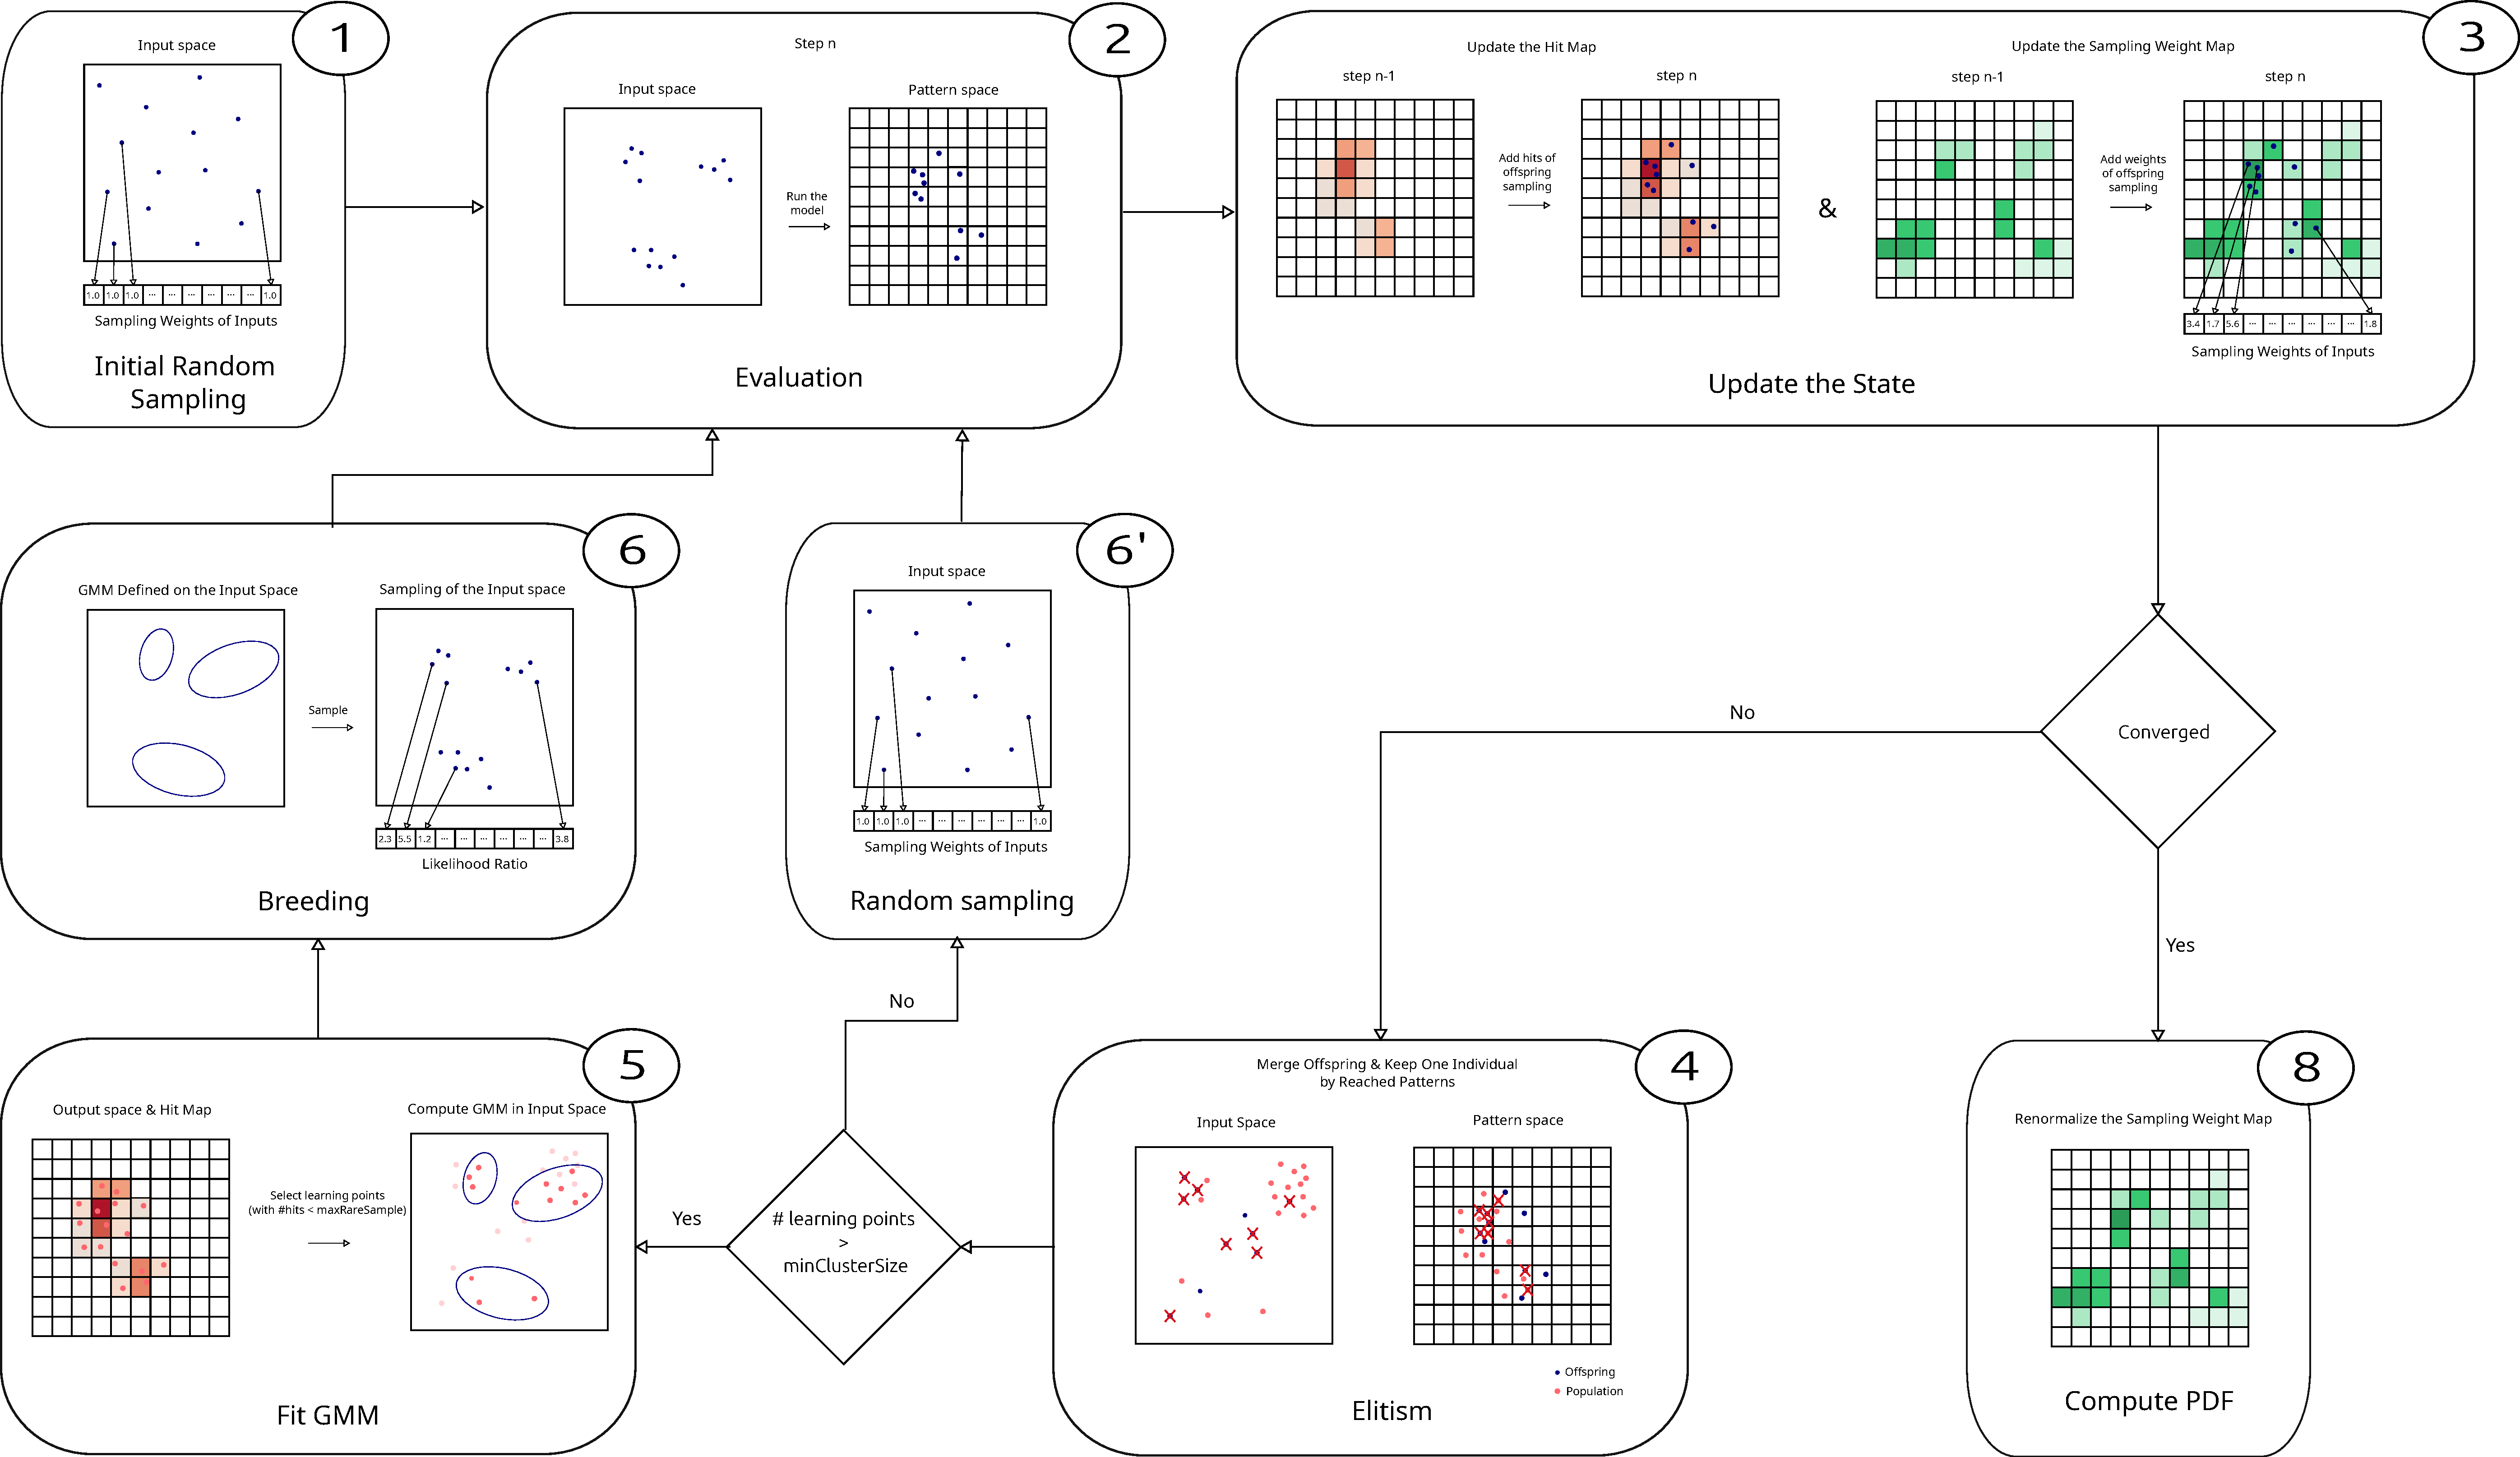
\includegraphics[width=0.8\linewidth]{images/schemaalgo.pdf}%{profils/zoomed/5.pdf}
 \captionof{figure}{ \label{SchemaAlgo} Graphical Representation of PPSE Algorithm }
\end{figure}


lambda

\subsection*{Patterns}

The PPSE algorithm has been developed in the frame of evolutionary algorithm. It computes the density of patterns that can be produced by the model. In the implementation of PPSE exposed in this paper we define a pattern as a vector of integral values. Generally the pattern are metrics that can be derived from the outputs of a model. For instance one can think of the discretisation by range of numerical values, some descriptors of temporal series such as the number of derivative sign change or the size of a population of agents. 

A given pattern can generally be produced by several (or an infinity) of input value for the model. The signature of a the pattern function provided to the algorithm is exposed in listing \ref{lst:pattern}. This function can for instance compute the output of a model for the input values x and then compute the pattern from the model outputs.

\begin{lstlisting}[caption={Pattern function},label={lst:patternFunction}]
def pattern(x: Vector[Double]): Vector[Int] = 
  // computation of the pattern for the point x
\end{lstlisting}


\subsection*{Algorithm State}\label{sec:algoState}

At each generation the population of solution is evolved. Additionally to this state, it maintains two pieces of state : a hit map and a density map. The data structures are exposed in listing \ref{lst:state}

The hit map contains the number of of times each pattern has been hit since the start of the algorithm. The density map contains the sum of the densities for each pattern: each time a pattern is hit, the density of the input point in the current GMM is summed in this the density map. 

\begin{lstlisting}[caption={State},label={lst:state}]
type LikelihoodRatioMap = Map[Vector[Int], Double]
type HitMap = Map[Vector[Int], Int]
\end{lstlisting}


\subsection*{Evolution Loop}

The evolution is the engine of the PPSE algorithm. It is a recursive function computing the successive states of the algorithm until a given number of generation has been exhausted. The code of the evolution loop is expose in listing \ref{lst:loop}.

The $evolution$ function takes the entire state of the algorithm as parameters. The 2 first parameters are the $genomes$ and the $patterns$ that have been computed for each of these genomes. These 2 parameters store the current population of solution of the evolutionary algorithm.

The next 2 parameters are the density map ($densityMap$) and the hit map ($hitMap$), described in section \ref{sec:algoState}.

The $gmm$ parameter passes the value of the GMM and the state of the rejection sampler. This is used in the breeding function to sample the new genomes and compute their densities.

The last 2 parameters are the random number generator ($random$) and the $generation$ number.

This function first test whether the number of generations is exhausted and the loop should be ended. In the case it is exhausted, it renormalises the densities and return a normalised density map. Otherwise it computes the next state of the algorithm.

The subsequent state is computed by first breeding $lamdba$ new genomes, then computing the pattern produced by each of these genomes. After that it calls the $elitism$ that keep the genomes producing pattern that are not present in the population already. Finally the function $updateState$ compute then new values for the hit map, then GMM and the density map and the evolution function is called recursively. Note that the computation of the GMM may fail in some degenerated configuration, in this case the previous GMM is preserved.

\begin{lstlisting}[caption={Evolution Loop},label={lst:loop}]
def evolution(
  genomes: Array[Array[Double]] = Array(),
  patterns: Array[Array[Int]] = Array(),
  likelihoodRatioMap: LikelihoodRatioMap = Map(),
  hitMap: HitMap = Map(),
  gmm: Option[(GMM, RejectionSamplerState)] = None,
  random: Random,
  generation: Int = 0): LikelihoodRatioMap =

  if generation >= generations
  then computePDF(likelihoodRatioMap)
  else
    val offSpringGenomes = breeding(genomeSize, lambda, gmm, random)
    val offspringPatterns = offSpringGenomes.map((g, _) => pattern(g.toVector, intervals).toArray)

    val (elitedGenomes, elitedPattern) =
      elitism(
        genomes = genomes, 
        patterns = patterns, 
        offspringGenomes = offSpringGenomes, 
        offspringPatterns = offspringPatterns)

    val (updatedHitMap, updatedlikelihoodRatioMap, updatedGMM) =
      updateState(
        genomes = elitedGenomes,
        patterns = elitedPattern,
        offspringGenomes = offSpringGenomes,
        offspringPatterns = offspringPatterns,
        likelihoodRatioMap = likelihoodRatioMap,
        hitMap = hitMap,
        fitOnRarest = 100,
        iterations = 1000,
        tolerance = 0.01,
        warmupSampler = 1000,
        minClusterSize = 10,
        random = random)

   evolution(elitedGenomes, elitedPattern, updatedlikelihoodRatioMap, updatedHitMap, updatedGMM orElse gmm, random, generation + 1)
\end{lstlisting}


\subsection*{Breeding}

The breeding function, exposed in listing \ref{lst:breeding}, produce new genomes sampled in the input space. It optional takes a GMM in parameter. In the first steps of the algorithm, while no GMM has been evaluated, it samples either uniformly. When the algorithm is advanced enough to construct a GMM (see section \ref{sec:updateState}) the breeding function sample in this GMM. It return the freshly sampled genomes and their respective densities. 

\begin{lstlisting}[caption={Breeding},label={lst:breeding}]
def breeding(
  genomeSize: Int,
  lambda: Int,
  gmm: Option[(GMM, RejectionSamplerState)],
  random: Random): Array[(Array[Double], Double)] =
  gmm match
    case None =>
      def randomGenome(size: Int, random: Random) = Array.fill(size)(random.nextDouble())
      Array.fill(lambda)((randomGenome(genomeSize, random), 1.0))
    case Some((gmm, rejectionState)) =>
      val rejectionSampler = buildRejectionSampler(gmm, random)
      val (_, samples) = sampleArray(rejectionSampler, lambda, rejectionState)
      samples
\end{lstlisting}


\subsection*{Elitism}

In genetic algorithms the elitism function generally shrinks the population by discarding the individual with the lowest fitness. In PPSE, only one individual by pattern is kept. The elitism function exposed in listing \ref{lst:elitism} keep only the first individual that has ever produced a given pattern.

\begin{lstlisting}[caption={Elitism function},label={lst:elitism}]
def elitism(
  genomes: Array[Array[Double]],
  patterns: Array[Array[Int]],
  offspringGenomes: Array[(Array[Double], Double)],
  offspringPatterns: Array[Array[Int]]): (Array[Array[Double]], Array[Array[Int]]) =

  def allGenomes = genomes ++ offspringGenomes.map(_._1)
  def allPatterns = patterns ++ offspringPatterns

  (allGenomes zip allPatterns).distinctBy { (_, pattern) => pattern }.unzip
\end{lstlisting}


\subsection*{Updating the State}\label{sec:updateState}

After the breeding, the evaluation and the elitism stages, the state of the algorithm is updated. Updating the state consists in computing the updated values for the hit map, the GMM and the density map. It is computed by the function $updateState$, exposed in listing \ref{lst:updateState}. 

This function first computes the new hit map. It simply increments the current number of hit by 1, for each pattern produced by the offspring.

The update State function then compute the new density map. To achieve this, it group the pattern in map, in with the keys are an offspring pattern and the value is a list of the densities of the offspring genomes which generated this pattern. The densities for a patterns are inverted and summed in the density map.

The third and last part of the state to be update is the GMM. Before updating the GMM, the function test if the algorithm is in bootstrapping phase. The bootstrapping phase occurs during the first few steps of the algorithm, while too few genomes have been evaluated to start fitting a GMM. While it is the case, the update state function return the newly computed hit map, the newly computed density map and no fitted GMM.

When enough genome are present in the population, a GMM is computed based on this genomes by the $computeGMM$ function. The computed GMM is returned along with the updated hit map and density map.

\begin{lstlisting}[caption={Update State},label={lst:updateState}]
def updateState(
  genomes: Array[Array[Double]],
  patterns: Array[Array[Int]],
  offspringGenomes: Array[(Array[Double], Double)],
  offspringPatterns: Array[Array[Int]],
  likelihoodRatioMap: LikelihoodRatioMap,
  hitMap: HitMap,
  fitOnRarest: Int,
  iterations: Int,
  tolerance: Double,
  warmupSampler: Int,
  minClusterSize: Int,
  random: Random): (HitMap, LikelihoodRatioMap, Option[(GMM, RejectionSamplerState)]) =
  def newHitMap =
    def updateHits(m: HitMap, p: Vector[Int]) = m.updatedWith(p.toVector)(v => Some(v.getOrElse(0) + 1))
    offspringPatterns.foldLeft(hitMap)((m, p) => updateHits(m, p.toVector))

  def newLikelihoodRatioMap =
    def offSpringDensities =
      val groupedGenomes = (offspringGenomes zip offspringPatterns).groupMap(_._2)(_._1)
      groupedGenomes.view.mapValues(v => v.map ((_, density) => 1 / density).sum).toSeq

    def updatePatternDensity(map: LikelihoodRatioMap, pattern: Array[Int], densitiy: Double): LikelihoodRatioMap =
      map.updatedWith(pattern.toVector)( v => Some(v.getOrElse(0.0) + densitiy))

    offSpringDensities.foldLeft(likelihoodRatioMap) { case (map, (pattern, density)) => updatePatternDensity(map, pattern, density) }

  if genomes.size < minClusterSize * 2
  then (newHitMap, newLikelihoodRatioMap, None)
  else
    def newGMM =
      computeGMM(
        genomes = genomes,
        patterns = patterns,
        hitMap = newHitMap,
        fitOnRarest = fitOnRarest,
        iterations = iterations,
        tolerance = tolerance,
        warmupSampling = warmupSampler,
        minClusterSize = minClusterSize,
        random = random
      )

    (newHitMap, newLikelihoodRatioMap, newGMM)
\end{lstlisting}


\subsection*{Computing the GMM}\label{sec:computeGMM}

At each step, the PPSE computes a GMM in order to sample the next generation. This GMM is fitted using the expectation maximisation (EM) algorithm {\color{red} ADD REF}. 

The computation of the GMM is exposed in listing \ref{lst:computeGMM}. The $computeGMM$ function selects the $fitOnRarest$ genomes,  with the lowest number of hits, in the current population. Then it clusterise these genomes using the $HDBSCAN$  algorithm {\color{red} ADD REF}. The result of the clustering is used to bootstrap the EM fitting algorithm (i.e. the $fitGMM$ function). 

In some edge cases, the $fitGMM$ function can fail to compute. In this case the $computeGMM$ function returns an empty option.

In general the $fitGMM$ function return a GMM. This GMM is framed in the boundaries of definition domain of the input space (in this case $[0,1]^n$). The framing is achieved by rejection, using a rejection sampler algorithm. The dilated GMM is returned.

\begin{lstlisting}[caption={Compute GMM},label={lst:computeGMM}]
def computeGMM(
  genomes: Array[Array[Double]],
  patterns: Array[Array[Int]],
  hitMap: HitMap,
  fitOnRarest: Int,
  iterations: Int,
  tolerance: Double,
  warmupSampling: Int,
  minClusterSize: Int,
  random: Random) =

  def rarestIndividuals = (genomes zip patterns).sortBy { case (_, p) => hitMap.getOrElse(p.toVector, 1) }.take(fitOnRarest)
  def rarestGenomes = rarestIndividuals.map(_._1)

  val (means, covariances, clusterWeights) = clusterize(rarestGenomes, minClusterSize, random)

  def initialGMM = GMM(means = means, covariances = covariances, weights = clusterWeights)

  fitGMM(
    x = rarestGenomes,
    gmm = initialGMM,
    iterations = iterations,
    tolerance = tolerance
  ) match
    case Success(newGMM) =>
      val rejectionSampler = buildRejectionSampler(newGMM, random)
      val samplerState = warmupSampler(rejectionSampler, warmupSampling)

      Some((newGMM, samplerState))
    case Failure(_) => None
\end{lstlisting}


\section*{Results}
% \section{Evaluation}
\label{sec. evaluation}

On évalue avec un modèle 2D => 2D car c'est facile à construire

On utilise (x, y) => (cauchy(x), cauchy(y))


On évalue la distance au téorique, avec la total variation distance. Il est possible que ça donne rien a cause des pattern communs. Si c'est le cas on pourra essayer de les exclure et de réapliquer la même meusure de distance.


% \section{Application}\label{sec. application}

\subsection*{The Squares Model}

\subsection*{The Hypercubes Model}

% \subsection*{The Flocking Model}
% \cite{Reynolds1987}


\subsection*{Traffic2Lanes}
The model "Traffic 2 Lanes"~\cite{wilensky1998netlogo} is based on NetLogo~\cite{wilensky1999netlogo}.

%In this section we consider $k\in\{1,\ldots, n\}$ to be fixed and we describe the CP algorithm for the analysis of the 
%$k$-th parameter. As mentioned earlier, the goal is to approximate $h_k(x)$, that is to provide 
%sufficiently good approximations of $h_k(a^j_k)$, for certain $a^1_k, \ldots, a^{l_k}_k \in A_k$. 
%
%In order to explore $A_k$ uniformly, we use an evolutionary algorithm with 
%diversity pressure mechanism \citep{Mouret2012b,Toffolo2003,Goldberg1992,Mahfoud1995}. Let $C_1, \ldots, C_{l_k}$ be $l_k$ different semantic 
%categories to which one can associate an element belonging to $A_k$. 
%In our approach, we consider that categories can be identified with intervals $I_1, \ldots, I_{l_k } \subseteq A_k$, and that 
%such intervals form a partition of $A_k$:
%
%\begin{enumerate}
%\item  $I_i \cap I_j = \emptyset$ if $i\neq j$, and 
%\item $\bigcup_{i=1}^{l_k} I_i= A_k$.
%\end{enumerate}
%
%We assume that these categories are good enough to characterize $A_k$, that is they are a good discretisation of $A_k$.
%For each $\alpha\in A_k$, we denote by $\mathfrak{cat}(\alpha)$ the category of $\alpha$, 
%that is the unique category $C_j$ such that $\alpha \in I_j$. We also denote by 
%$\mathfrak{Cat} : A \rightarrow \{C_1, \ldots, C_{l_k}\}$ the map defined by 
%$\mathfrak{Cat}(\bar{a})= \mathfrak{cat}(a_k)$, where $\bar{a} = (a_0, \ldots, a_{n-1})$; 
%it defines the category of a parameter vector as the category of its $k$-th coordinate.
%The algorithm is devised to find parameter vectors   $\{\bar{a}^1, \ldots, \bar{a}^{l_k}\}$,  
%with $\bar{a}^j = (a^j_1, \ldots, a^j_{n})$ and $a^j_i\in A_i$, such that:
%
%\begin{enumerate}
%\item Each vector lies in a different category:  $\mathfrak{Cat}(\bar{a}^j) = C_j$ for $j = 1\ldots l_k$. This means 
%that, when projecting on the $k$-th coordinate, our sample is representative of the whole space $A_k$.
%
%\item For each $\bar{a}^j$, the value of $f(\bar{a}^j)$ is a good approximation of $h_k(\bar{a}^j)$.
%
%
%\end{enumerate}
%
%
%The idea of the algorithm is to generate successive sets of solutions and to keep only the best solution per category. 
%At each iteration the set of best solutions is updated. 
%


%\bigskip
%The algorithm is composed of the following steps:
%
%\paragraph{Initialization.} We construct an initial set of parameter vectors.
%
%\subparagraph{Step 0.} 
%We first generate a random set $X_0$  of parameter vectors, that is $X_0 = \{\bar{a}^1, \ldots, \bar{a}^{M}\}$,  
%with $\bar{a}^j = (a^j_1, \ldots, a^j_{n})$ and $a^j_i\in A_i$. The number $M$ may be much higher than $l_k$.
%
%
%\medskip
%\paragraph{Approximation loop.}
%
%We construct $X_{N+1}$ from $X_N$.
%
%
%\subparagraph{Step 1.} 
%We construct the sets $S_i = \{\bar{a}\in X_N: \mathfrak{Cat}(\bar{a})= C_i \} $ for $i= 1, \ldots,l_k$ (we may get $S_i = \emptyset$).
%
%\subparagraph{Step 2.}
%Here we apply elitism, that is we select only the best parameter vector in each category: We construct the sets 
%$E_i = \{ \bar{a}\in S_i : f(\bar{a})\leq f(\bar{a}') \mbox{ }\forall \bar{a}'\in S_i\}$ for $i= 1, \ldots,l_k$, and 
%$H = \bigcup_{i=1}^{l_k} E_i$. 
%In practice all the sets $E_i$ will be either empty (if $S_i=\emptyset$) 
%or composed by only one parameter vector;  if there exist more more than one that are minimal in $S_i$, then we can 
%randomly choose a fixed number of them to compose $E_i$.
%
%
%\subparagraph{Step 3.}
%Generate $H^*$ from $H$ by randomly modifying the parameter vectors in $H$. 
%We can for instance generate each vector in $H^*$ by applying a gaussian variation to a vector in $H$.   
%
%\subparagraph{Step 4.}
%Define the set $X_{N+1}$ as the union of $H$ and $H^*$. Check if a predefined stopping criterion is met 
% (number of iterations, stabilization of the solutions, etc.): Go to Step 5 if it is, iterate Steps 1 to 4 if is not. 
%
%\paragraph{Ending.} 
%When the stopping criterion is met, we can output our approximation to the function $h_k(x)$.
%
%\subparagraph{Step 5.} 
%If $\{\bar{a}^1, \ldots, \bar{a}^m\}$ is the last $H$ computed,  we define our approximation to  $h_k(x)$ as the set of 
%$2$-tuples $\{(\bar{a}^1_k, f(\bar{a}^1)), \ldots,(\bar{a}^m_k, f(\bar{a}^m)) \}$. Let us note that by construction $m \leq l_k$, 
%but in practice, when the number of iterations is high enough (see section \ref{sec. validityAlgo}), 
%we get $m = l_k$.




\section*{Discussion}
\subsection*{Validity}\label{sec. validityAlgo}
%As we said in section \ref{sec. objective}, our approach consists in estimating the impact of the $k$-th parameter on 
%the performance of the model, by finding a good approximation to the function $h_k(x)$. 
%To clarify why our method provides indeed such a good approximation, we make the following remarks: 
%
%\begin{enumerate}
%\item At each iteration we randomly generate new solutions from old ones. Given a solution $\bar{a}$ such that 
%that $\mathfrak{C}(\bar{a}) = C_j$, the probability of getting a new solution $\bar{a}'$ from $\bar{a}$ such that  
%$\mathfrak{C}(\bar{a}') = C_{j'}$, with $j' \neq j $, is different from $0$ (this is clearly the case if we use, for instance, 
%a gaussian variation). Hence, if enough iterations are repeated, every category will eventually be reached by as 
%many solutions as we wish.
%
%\item Let us consider 
%$\alpha =\inf\{f (\bar{a}): \mathfrak{Cat}(\bar{a}) = C_j\} = 
%\inf \{h_k(a): \mathfrak{cat}(a) = C_j\}$. 
%If the $f$ is sufficiently regular (it is enough if it is continuous, or if it is just semi-continuous on its local minima), 
%then, by the analogous argument to that in point 1.,  we will eventually find an solution $\bar{a}$ such that 
% $ \mathfrak{Cat}(\bar{a}) = C_j$  and $f(\bar{a})$ is as close to $\alpha$ as we want.
%
%\end{enumerate} 
%
%\smallskip
%These remarks, together with the fact that we can consider as many categories as needed, justify our claim. 
%We should note that, as it is usually the case with evolutionary algorithms, we do not provide a precise speed 
%of convergence for our algorithm; however, experimental results are very satisfactory (see section \ref{application}).

\subsection*{Extensions of the algorithm}\label{sec. extensions}

Application to stochastic problems

Other distributions for inputs


%In section \ref{sec. algoDescription}  we have presented the most basic version of our algorithm, for the sake of clarity. 
%However in practice we use a variation of it, heuristically devised, to improve its performance. 
%In this section we present these modifications. We use the same notation as in section \ref{sec. algoDescription}.
%
%The main point of this modified version is the random generation of new solutions (step 3). 
%In this part we rely on the standard techniques used in genetic algorithms, in which the random variation comes from 
%two biologically-inspired operators: \emph{mutation} and \emph{crossover}. These operators are not applied to the 
%whole set $H$ of solutions, but rather on a subset $H_0\subseteq H$ which is generated by a certain 
%\emph{selection} mechanism (we will explain below this selection mechanism). 
%From $H_0$ we generate $H^*$ in two steps: We first generate a new set of solutions $H'_0$ by applying a $SBX$-crossover 
%to $H_0$ (see \citep{Deb1994}), and then we apply a self-adapting Gaussian mutation to $H'_0$ (see \citep{Hinterding1995}). 
%The result will be our $H^*$.
%
%In the generation of $H_0\subseteq H$ we follow a standard selection mechanism: Binary tournament selection. 
%It consists in randomly choosing two solutions $x, y \in H$, comparing them via a certain function 
%$g: H \rightarrow \mathbb{R}\cup\{\infty\}$ and then keeping the best ($x$ is kept if $g(x)\geq g(y)$); we repeat this procedure 
%until we reach the desired size of $H_0$. 
%
%\smallskip
%\begin{nt*}
%Although we have defined $H_0$ as a set (elements in $H_0$ are unique), we can also define $H_0$ as a tuple, 
%allowing then a same solution to appear more than once.
%\end{nt*}
%
%One feature that is specific to our approach is the definition of the function $g$, that we call \emph{local contribution}.
%
%\begin{df*}
%Let $H = \{\bar{a}^1, \ldots, \bar{a}^m\}$ and $\bar{a}^1< \ldots < \bar{a}^m$. 
%Given a solution  $\bar{a}^j\in H\setminus\{\bar{a}^1, \bar{a}^m\}$, let $\Delta_j$ denote
%the area of the triangle in $\mathbb{R}^2$ formed by the $2$-tuples 
%$(\bar{a}^{j-1}_k, f(\bar{a}^{j-1}))$, $(\bar{a}^{j}_k, f(\bar{a}^{j}))$ and $(\bar{a}^{j+1}_k, f(\bar{a}^{j+1}))$ . 
%Then we define the \emph{local contribution of} $\bar{a}^j$, as 
%$$g(\bar{a}^j) =(-1)^{\varepsilon}\Delta_j,$$ 
%where 
%$\varepsilon = 0$ if the point $(\bar{a}^{j}_k, f(\bar{a}^{j}))$ is below the straight line from
%$(\bar{a}^{j-1}_k, f(\bar{a}^{j-1}))$ and $(\bar{a}^{j+1}_k, f(\bar{a}^{j+1}))$, and $\varepsilon = 1$ if it is not.
%If $\bar{a}^j$ is extreme, i.e. $\bar{a}^j\in \{\bar{a}^1, \bar{a}^m\}$, then we define $g(\bar{a}^j) = \infty$.
%\end{df*}
%
%We have just described how to generate a new set of solutions $H^*$ from $H$. The heuristics behind this 
%procedure is to give some priority to the generation of new solutions that are either locally good, which accelerates 
%the approximation to the local minima in each category, or on the extremes, which widens the exploration of 
%the space. 
%
%\smallskip
%In order to describe the version of the algorithm that we use in experiments, the other point we should mention is 
%the stopping criterion. A natural choice would be based on the stability of the successive $H$ computed: If we detect 
%no important changes from one $H$ to the next one (during several iterations), the algorithm stops. 
%We can measure these changes in different ways, for instance considering the function 
%$F(H) = \sum_{\bar{a}\in H} f(\bar{a})$. However, in practice, we consider a maximal computation time as the stopping 
%criterion and the stability becomes an element of subsequent analysis.

%\subsection*{Generic implementation}

%In order to make the CP algorithm usable we provide along with this paper a generic implementation in the free and open source library called MGO (Multi Goal Optimisation)\footnote{https://github.com/ISCPIF/mgo} programmed in Scala\footnote{http://scala-lang.org/}. MGO is a flexible library of evolutionary algorithms. It leverages the Scala "trait" system to provide a high level of modularity.
%
%This section shows how to compute a calibration profile on a toy model with MGO. In this example, the model is the Rastrigin function and the objective is to minimise this function. The objective function in MGO should be implemented through a specialised trait of the "Problem" trait. Listing \ref{lst:rastrig} shows how to implement the Rastrigin function into MGO.
%
%\lstinputlisting[caption={Implementation of the Rastrigin function in MGO},label={lst:rastrig}]{rastrig.scala}
%
%To compute a calibration profile of this Rastrigin function it should be composed with the "Profile" trait that provides the CP algorithm. Listing \ref{lst:rastrigprofile} expose how to achieve this composition. In this example two other traits are used: A termination criterion based on a maximum number of step ("CounterTermination") and a trait to specify that the profile is computed on a part of the genome ("ProfileGenomePlotter").
%
%\lstinputlisting[caption={Computing the profile of the Rastrigin function in MGO},label={lst:rastrigprofile}]{rastrigprofile.scala}
%
%Like most evolutionary algorithm, the CP algorithm compute the evaluation function many times. Those numerous evaluations could be computationally costly. MGO is therefore naturally parallel and takes advantage of all the cores of the central processing units. This kind of parallelism is suitable for many models but can be limiting in case of large stochastic agent based models for instance. To overpass this limit we have integrated the CP algorithm in the OpenMOLE\footnote{www.openmole.org} (Open Model Exploration) framework \citep{Reuillon2013}. OpenMOLE enables the distribution of the CP algorithm on large scale distributed computing infrastructures including multi-core computers, computing clusters and even world wide computational grid. In the following section we used this distributed implementation of CP framework to study a real world agent based model.

%\section{Application the SimpopLocal geographical model}
%\label{application}
%
%\subsection*{A model to simulate the emergence of structured urban settlement system}

%SimpopLocal is a stylized model of an agrarian society in the Neolithic period, during the primary ``urban transition'' manifested by the appearance of the first cities \citep{schmitt2014}. It is designed to study the emergence of a structured and hierarchical urban settlement system by simulating the growth dynamics of a system of settlements whose development remains hampered by strong environmental constraints that are progressively overcome by successive innovations. This exploratory model seeks to reproduce a particular structure of the Rank-Size distribution of settlements well defined in the literature as a generalized stylized-fact: For any given settlement system throughout the time and continents, the distribution of sizes is strongly differentiated, exhibiting a very large number of small settlements and a much smaller number of large settlements \citep{archaeomedes1998, berry1964, fletcher1986, liu1996}. This kind of distributions can be modeled by a power-law when small settlements are not considered or a log-normal when small settlements are considered \citep{robson1973, favaro2011}. Such distributions are easily simulated by rather simple and non spatial statistical stochastic models \citep{gibrat1931, simon1955}. But for theoretical considerations and to specify the model in a variety of geographical frames, we think it necessary to make explicit the spatial interaction processes that generate the evolution of city systems. According to the evolutionary theory of system of cities \citep{pumain2009c, Pumain1997b}, the growth dynamics of each settlement is controlled by its ability to generate interurban interactions. The multi-agent system modeling framework enables us to include mechanisms, derived from this theory, that govern the interactions between settlements \citep{bretagnolle2006, pumain2013}. The application of this concept resulted in several Simpop models \citep{bretagnolle2010, bura1996, sanders1997} in which the expected macro-structure of the log-normal distribution of sizes emerges from the differentiated settlement growth dynamics induced by the heterogeneous ability of interurban interactions. Therefore the aim of SimpopLocal is to simulate the hierarchy process via the explicit modelling of a growth distribution that is not entirely stochastic as in the Gibrat model \citep{gibrat1931} but that emerges from the spatial interactions between micro-level entities.

%\subsection*{Agents, attributes, and mechanisms of the model}

%The SimpopLocal model is a multi-agent model developed with the Scala software programming language. The landscape of the simulation space is composed of a hundred of settlements. Each settlement is considered as a fixed agent and is described by three attributes: The location of its permanent habitat, the size of its population, and the available resources in its local environment. The amount of available resources is quantified in units of inhabitants and can be understood as the carrying capacity of the local environment for sustaining a population. This carrying capacity depends on the resources exploitation skills that the local population has acquired from inventing or acquiring innovation. Each new innovation acquired by a settlement develops its exploitation skills. This resource exploitation is done locally and sharing or trade is not explicitly represented in the model.
%The growth dynamics of a settlement is modelled according to the assumption that its population size is dependent on the amount of available resources in the local environment and is inspired from the Verhulst model \citep{verhulst1845} or logistic growth. For this experiment, we assume a continuous general growth trend for population - this may be different in another application of the model. The annual growth factor $r_{growth}$ is expressed on an annual basis, thus one iteration or step of the model simulates one year of demographic growth. $r_{growth}$ has been empirically estimated to $0.02$. The limiting factor of growth  $R_{M}^{i}$ is the amount of available resource that depends on the number $M$ of innovations the settlement $i$ has acquired by the end of the simulation step $t$. $P_{t}^{i}$ is the population of the settlement $i$ at the simulation step $t$:
%
%\[ P_{t+1}^{i}= P_{t}^{i}.[1+r_{growth}. (1-\dfrac{P_{t}^{i}}{R_{M}^{i}})] \]
%
%The acquisition of a new innovation by a settlement allows it to overtake its previous growth limitation by allowing a more efficient extraction of resources and thus a gain in population size sustainability. With the acquisition of innovations the amount of available resources tends to the maximal carrying capacity $R_{max}$ of the simulation environment:
%
%\[ R_{M}^{i}
%\overset{Innovation Acquisitions}{\longrightarrow}
%R_{max}\]
%
%The mechanism of this impact follows the Ricardo model of diminishing returns, also a logistic model \citep{turchin2003}. The $InnovationImpact$ parameter represents the impact of the acquisition of an innovation and has a decreasing effect on the amount of available resources  $R_{M}^{i}$  with the acquisition of innovations:
%
%\[R_{M+1}^{i}= R_{M}^{i}.[1+ InnovationImpact.(1-\dfrac{R_{M}^{i}}{R_{max}})] \]
%
%
%Acquisition of innovations can occur in two ways, either by the emergence of innovation within a settlement or by its diffusion through the settlement system. In both cases, interaction between people inside a settlement or between settlements is the driving force of the dynamics of the settlement system. It is a probabilistic mechanism, depending on the size of the settlement. Indeed, innovation scales super-linearly: The greater the number of innovations acquired, the bigger the settlement and the higher the probability of innovating \citep{arthur2009, diamond1997, lane2009}. To model the super-linearity of the emergence of innovation within a settlement, we model its probability by a binomial law. If $P_{creation}$ is the probability that the interaction between two individuals of a same settlement is fruitful, i.e. leads to the creation of an innovation, and $N$ the number of possible interactions, then by the binomial law, the probability of the emergence of at least one innovation $P_{m_{creation}>0})$  can be calculated and then used in a random drawing :
%
%
%\[ \Pi_{m_{creation}>0} = 1 - P_{m = 0}\]
%\[ \Pi_{m_{creation}>0} = 1-[ \dfrac{N!}{0!(N-0)!}.P_{creation}^{0}.(1-P_{creation})^{N-0}] \]
%\[ \Pi_{m_{creation}>0} = 1-(1-P_{creation})^{N}\]
%
%If the size of the settlement $i$ considered is  $P_{t}^{i}$  then the number $N$ of possible interactions between individuals of that settlement is:
%
%\[ N = \frac{P_{t}^{i}.(P_{t}^{i}-1)}{2}\]
%
%The diffusion of an innovation between two settlements depends both on the size of populations and the distance between them. If $P_{diffusion}$ is the probability that the interaction of two individuals of two different settlements is fruitful, i.e. leads to the transmission of the innovation, and $K$ the number of possible interactions, then by the Binomial law the probability of diffusion of at least one innovation $P(m_{diffusion} >0)$  can be calculated and used in a random drawing :
%
%\[ \Pi_{m_{diffusion}>0} = 1-(1-P_{diffusion})^{K}\]
%
%But in this case, the size $K$ of the total population interacting is a fraction of the population of the two settlements $i$ and $j$ which is decreasing by a factor $DistanceDecay$ with the distance $D_{ij}$ between the settlements, as in the gravity model \citep{wilson1971}:
%
%\[K = \dfrac{1}{2}.\dfrac{P_{t}^{i}.P_{t}^{j}}{D_{ij}^{DistanceDecay}} \]
%
%However another mechanism controls this innovation diffusion process. Each innovation can only be diffused during a time lap just after its acquisition by a settlement. This time lap of diffusion is controlled by the parameter $InnovationLife$. According to this deprecation mechanism, an innovation is considered obsolete after $InnovationLife$ simulated years and cannot be diffused any more.
%
%SimpopLocal involves six free parameters that cannot be evaluated using empirical values: $InnovationLife$, $InnovationImpact$, $R_{max}$, $P_{creation}$, $P_{diffusion}$, $DistanceDecay$. Those parameter are constraints by the definition domains shown in Table \ref{tab:DefinitionBoundaries}.
%
%\begin{table}[h]
%\begin{center}
%\begin{tabular}{|c|c|c|}
%
%\hline 
%Parameter & Definition domain \\ 
%\hline 
%$R_{max}$ & $[1; 40,000]$ \\ 
%\hline 
%$InnovationImpact$ & $[0; 2]$ \\ 
%\hline 
%$P_{creation}$ & $[0; 0.1]$ \\ 
%\hline 
%$P_{diffusion}$ & $[0; 0.1]$ \\ 
%\hline 
%$DistanceDecay$ & $[0; 4]$ \\ 
%\hline 
%\end{tabular}   
%\caption{Definition boundaries for SimpopLocal parameters}\label{tab:DefinitionBoundaries}
%\end{center}
%\end{table}
%
%In order to ensure the replicability of the model, a portable implementation has been designed and the source code of SimpopLocal used in this experiment has been filed in a public repository \footnote{https://github.com/ISCPIF/profiles-simpoplocal}.

%\subsection*{Objective function}

%As defined in section \ref{sec. objective} the CP method requires the definition of the $f$ objective function that evaluates a set of parameter values by computing a scalar value (the lowest this value is the better the set of parameter values). For SimpopLocal, $f$ aggregates three objective functions to assess the ability of SimpopLocal to reproduce the stylized facts that we seek to simulate for a given set of the parameter values. 
%
%The SimpopLocal model being stochastic, the simulation outputs vary from one simulation to the next for a given parameter setting. Therefore, the evaluation of the parameter settings on the three objectives must take into account this variability. Each evaluation is therefore computed on the output of 100 simulations. We have shown in \citep{schmitt2014} that it was a suitable compromise between capturing the variability and not increasing to much the computation duration. Here is how we test each set of parameters according to the three objective functions:
%\begin{itemize}
%\item The objective of distribution quantifies the ability of the model to produce settlement size distributions that fit a log-normal distribution. First we evaluate the outcome of each subset of 100 simulations corresponding to one parameter setting by computing, according to a 2-sample Kolmogorov-Smirnov test, the deviation between the simulated distribution and a theoretical log-normal distribution having the same mean and standard deviation. Two criteria are reported, with value 1 if the test is rejected and 0 otherwise: The likelihood of the distribution (the test returns 0 if $p-value > 5\%$) and the distance between the two distributions (the test returns 0 if $D-value < D\alpha$). In order to summarize those tests in a single quantified evaluation, we add the results of the two tests on the 100 simulations. The best possible score on this objective is thus 0 (all tests returning 0) and the worst 200 (all tests returning 1). By dividing this score by the worst possible value (200), we get a normalised error objective noted $o1$. 
%
%\item The objective of population (noted $o2$) quantifies the ability of the model to generate large settlements that have an expected size. The outcome of one simulation is tested by computing the deviation between the size of the largest settlement and the expected value of 10,000 inhabitants: (\textit{populationOfLargestSettlement} - 10000) / 10000. The evaluation of the parameter setting reports the median of this test on the 100 simulations. 
%
%\item The objective of simulation duration (noted $o3$) quantifies the ability of the model to generate an expected configuration in a suitable length of time (in simulation steps). The duration of one simulation is tested by computing the deviation between the number of step of the simulation and the expected value of 4000 simulation steps: (\textit{simulationSteps} - 4000) / 4000. The evaluation of the parameter setting reports the median of this test on the 100 simulations.
%\end{itemize}
%
%Given these three objectives, $f$ is defined as an aggregated objective value that summarises the calibration error of a set of parameter values. This summarized objective is defined as: $f = max(o1, o2, o3)$. The lowest $f$ is, the better a set of parameter values.
%
%To analyse the produced results, we have established that only input parameters leading to values of $f$ of less than $0.1$ of error are considered valid. Indeed, the empirical data and theoretical knowledge that led to the definition of the objective function are not precise enough to justify a more thorough analysis of the model. This threshold is largely exceeded for some parameter values, however rendering this threshold  of acceptability explicit enables the definition of credible bounds for each of the free parameter of the model. These bounds define a validity domain of each of the parameters. Note that the profile algorithm iteratively refines the computed profiles from high values toward lower ones through through an iterative process, therefore the proposed bounds are more restrictive than the exact ones.

%\subsection*{Results}

%This section exposes results of the CP algorithm on each of the six free parameters of SimpopLocal. Each profile presented in this paper has required the achievement of 100,000 CPU hours time (meaning that it would have required 100,000 hours of computation on a single core of a modern processor). To achieve such a huge computational load we have distributed it across the numerous CPU of the European computation grid EGI (European Grid Infrastructure) using the distributed implementation of CP that we have integrated into OpenMOLE. The effective user time was around 15 days to compute all the profiles achieving a gain of 2200. The OpenMOLE script files used to compute those profiles have been made available\footnote{https://github.com/ISCPIF/profiles-simpoplocal}. 
%
%
%\subsubsection{$InnovationLife$}
%
%The value of the parameter $InnovationLife$ depicts the duration during which an innovation can diffuse in the system of settlements. The Figure \ref{InnovationLifeProfile} shows the application of the CP algorithm this parameter. When $InnovationLife$ is set to 0 the model can not be calibrated. For such a value the innovations are instantly deprecated just after their creation, meaning that no diffusion of innovation is possible. This particular point shows that the diffusion process of the model is mandatory to produce acceptable dynamics.
%
%\begin{figure}
% \centering
%  \includegraphics[width=0.8\linewidth]{profil-phdClara/InnovationLife.pdf}%{profils/zoomed/5.pdf}
% \captionof{figure}{ \label{InnovationLifeProfile} Calibration profile of the parameter $InnovationLife$ }
%\end{figure}
%
%Under the value 150 the calibration error is higher than our validity threshold and there for we consider that the model cannot be calibrated. From a thematical point of view: The deprecation of the innovations is too fast, thus the innovations cannot percolate in the system leading to unrealistic dynamics.
%
%Over the value 150 the obsolescence of the innovations is slow enough to have no noticeable effect on the calibration of the model. In particular when $InnovationLife$ is set to 4000, the calibration error is lower than our acceptance threshold. For this particular value, the matching mechanism of innovation obsolescence could be considered as disabled: The maximum duration of a simulation is 4000 steps, therefore when $InnovationLife$ is set to 4000, the innovations are never considered deprecated. This profile shows that this mechanism does not constrain much the model and is useless to reproduce the expected dynamics. Seeking for a more parsimonious model we have removed this mechanism. The following of the article is based on the SimpopLocal model without the deprecation mechanism. 
%
%\subsubsection{$R_{max}$}
%
%The parameter $R_{max}$ constraints the maximum size of settlements by limiting the impact of the acquisition of an innovation on the size of a settlement. The calibration profile for this parameter is shown on Figure \ref{RMaxProfile}.
%
%\begin{figure}
% \centering
%  \includegraphics[width=0.8\linewidth]{profil-phdClara/Rmax.pdf} %{profils/zoomed/0.pdf}
% \captionof{figure}{ \label{RMaxProfile} Calibration profile of the parameter $R_{max}$ }
%\end{figure}
%
%The calibration objective for the size of the biggest settlement has been set to 10,000 inhabitants. When $R_{max}$ is set to a value lower than 10,000 it is impossible for the model to reach the 10,000 population objective. Thus, by construction, low values of this parameter can not achieve acceptable calibration errors.
%
%The profile exposes a narrowed range of very low calibration error between $[9500; 10500]$. Surprisingly the calibration algorithm is not able to find low calibration errors for $R_{max}$ above 10,500. It indicates that this mechanism is necessary to produce acceptable dynamics and reaching settlements of a size matching empirical evidences.
%
%\subsubsection{$InnovationImpact$}
%
%The $InovationImpact$ parameter controls the impact of the acquisition of an innovation on the growth of a settlement. The Figure \ref{InnovationImpactProfile} show the calibration profile for this parameter. The section of the profile containing low calibration errors is very narrowed, only 2 solutions with calibration errors under 0.1 have been found. This profile has been computed using the definition domain provided by the modellers $[0; 2]$. From the Figure \ref{InnovationImpactProfile} it can be deduced that the definition domain is too wide compared to the validity domain for this parameter. Therefore another profile has been computed for a much more restraint definition domain: $[0; 2.10^{-2}]$.
%
%\begin{figure}
% \centering
%  \includegraphics[width=0.8\linewidth]{profil-phdClara/InnovationImpact.pdf} %profils/large/4.pdf
% \captionof{figure}{ \label{InnovationImpactProfile} Calibration profile of the parameter $InnovationImpact$ }
%\end{figure}
%
%
%The zoomed profile is shown on Figure \ref{DetailedInnovationImpactProfile}. It shows that when the impact on the settlement growth of the innovation is too low the dynamic is too slow to reach the calibration objectives. On the contrary, when $InnovationImpact$ is too high the growth of the settlements is too fast to match credible dynamics (whatever the value of the other parameters can be). This profile shows that the validity domain of this parameter is $[0.006; 0.01]$.
%
%\begin{figure}
% \centering
%  \includegraphics[width=0.8\linewidth]{profil-phdClara/InnovationImpactZ.pdf} %{profils/zoomed/4.pdf}
% \captionof{figure}{ \label{DetailedInnovationImpactProfile} Detailed calibration profile of the parameter $InnovationImpact$ }
%\end{figure}
%
%\subsubsection{$P_{creation}$}
%
%The $P_{creation}$ parameter determines the capacity of a settlement to create a new innovations. The Figure \ref{pCreationProfile} shows the calibration profile for this parameter. Once again the definition domain given by the modellers $[0; 0.01]$ is too wide to establish directly a validity domain. However, this profile shows that for high values of $P_{creation}$ the model can not reach low calibration errors. The inflexion of the profile near the value 0 indicates that low calibration errors are located in a much more narrowed domain close to 0.
%
%\begin{figure}
% \centering
%  \includegraphics[width=0.8\linewidth]{profil-phdClara/Pcreation.pdf}%{profils/large/2.pdf}
% \captionof{figure}{ \label{pCreationProfile} Calibration profile of the parameter $P_{creation}$ }
%\end{figure}
%
%The Figure \ref{DetailedpCreationProfile} shows the calibration profile of the $P_{creation}$ parameter within the domain $[0; 1e^{-5}]$. From this profile it can be deduced that the validity domain of $P_{creation}$ is $[0.4\times10^{-6}; 2\times10^{-6}]$. For low values of $P_{creation}$ the model can not be calibrated. The innovations are generated too slowly to engender a sufficient growth (whatever the value of the other parameters can be). For high values of $P_{creation}$ the system races and growth is too fast.
%
%\begin{figure}
% \centering
%  \includegraphics[width=0.8\linewidth]{profil-phdClara/PcreationZ.pdf}%{profils/zoomed/2.pdf}
% \captionof{figure}{ \label{DetailedpCreationProfile} Detailed calibration profile of the parameter $P_{creation}$ }
%\end{figure}
%
%
%
%\subsubsection{$P_{diffusion}$}
%
%The parameter $P_{diffusion}$ governs the exchange of innovation between settlements. The Figure \ref{pDiffusionProfile} shows the calibration profile for this parameter which is very flat and contains only high calibration errors. This profile exposes a shortcoming of the algorithm. If the definition domain is very wide compared to the validity domain, the method might take a lot of computation time to find the parameters settings matching low calibration errors and give the false impression that they don't exist. In the case of SimpopLocal we know that low calibration errors exists because they were found when computing the other profiles. By deduction from the model mechanisms, low calibration errors should be found in a domain closer to 0.
%
%\begin{figure}
% \centering
%  \includegraphics[width=0.8\linewidth]{profil-phdClara/Pdiffusion.pdf} %{profils/large/3.pdf}
% \captionof{figure}{ \label{pDiffusionProfile} Calibration profile of the parameter $P_{diffusion}$ }
%\end{figure}
%
%The zoomed profile using the definition domain $[0; 10^{-5}]$ is shown on Figure \ref{DetailedpDiffusionProfile}. At this scale the validity domain containing a single interval appears: $[0.3\time10^{-6} ; 1.8\time10^{-6}]$. 
%
%\begin{figure}
% \centering
%  \includegraphics[width=0.8\linewidth]{profil-phdClara/PdiffusionZ.pdf} %{profils/zoomed/3.pdf}
% \captionof{figure}{ \label{DetailedpDiffusionProfile} Detailed calibration profile of the parameter $P_{diffusion}$ }
%\end{figure}
%
%A very interesting aspect of this profile is that low values of $P_{diffusion}$ prevent the model from producing acceptable dynamics. Noticeably when $P_{diffusion} = 0$ it disables entirely the diffusion mechanism of the model. At this particular point the calibration error is unsatisfying, thus this profile shows that the diffusion mechanism is mandatory in order to produce realistic behaviours.
%
%\subsubsection{$DistanceDecay$}
%
%The parameter $DistanceDecay$ acts on the mechanism of diffusion of the innovations. It introduces a decaying effect of the distance between settlements on the probability to diffuse an innovation from one settlement to another. Figure \ref{DistanceDecayProfile} shows the calibration profile for this parameter. High values of this parameter prevent the diffusion. The calibration errors computed with high values of $DistanceDecay$ are almost equal to the calibration errors computed with $P_{diffusion}$ set to 0 (that also inhibits the diffusion process). This indicates both the coherence of the model and of the method. 
%
%
%\begin{figure}
% \centering
%  \includegraphics[width=0.8\linewidth]{profil-phdClara/DistanceDecay.pdf} %{profils/zoomed/1.pdf}
% \captionof{figure}{ \label{DistanceDecayProfile} Calibration profile of the parameter $DistanceDecay$ }
%\end{figure}
%
%The validity domain of $DistanceDecay$ is [0.2, 1.1]. The mechanism piloted by $DistanceDecay$ introduces a distance effect in the interaction process creating spatial heterogeneity. For low values of $DistanceDecay$ the profile shows only unsatisfying calibration errors. It means that spatial heterogeneity is mandatory to produce acceptable dynamics. 

\section*{Conclusion}

%This paper proposes a new method to explore models. This method called CP computes 2-dimensional graphs that depict the effect of each parameter on the ability of a model to produce expected dynamics. This method has been shown very useful to better understand the dynamical behaviours of a geographical multi-agent simulation model. Using the CP method on this model important novel understandings are deduced:
%\begin{itemize}
%\item The mechanism linked to the parameter $InnovationLife$ of the model has been shown useless. This mechanism has thus been removed from the model, making it more parsimonious,
%\item except from this mechanism all the other mechanisms (i.e spatial heterogeneity, diffusion of the innovations, creation of the innovations...) have been shown mandatory to produce acceptable dynamics,
%\item for the all parameters (except from $InnovationLife$) a connected validity domain has been proposed, these boundaries are summarised on Table \ref{tab:Boundaries}. 
%\end{itemize}
%
%\begin{table}[h]
%\begin{center}
%\begin{tabular}{|c|c|c|c|}
%
%\hline 
%Parameter & Definition domain & Validity domain \\ 
%\hline 
%$R_{max}$ & $[1; 40,000]$ & $[9,500; 11,500]$ \\ 
%\hline 
%$InnovationImpact$ & $[0; 2]$ & $[6\times10^{-3}, 1\times10^{-2}]$ \\ 
%\hline 
%$P_{creation}$ & $[0; 0.1]$ & $[4\times10^{-7}; 2\times10^{-6}]$ \\ 
%\hline 
%$P_{diffusion}$ & $[0; 0.1]$ & $[3\times10^{-7}; 8\times10^{-6}]$ \\ 
%\hline 
%$DistanceDecay$ & $[0; 4]$ & $[0.2; 1.1]$ \\ 
%\hline 
%\end{tabular}   
%\caption{Validity boundaries for SimpopLocal parameters}\label{tab:Boundaries}
%\end{center}
%\end{table}

\section*{Acknowledgments}

\nolinenumbers

\bibliography{ppse}

\end{document}